Para facilitar a programação do microcontrolador será feito o uso da biblioteca TivaWare fornecida pela Texas Instruments. Tal ferramenta facilita o controle do processador e acesso aos periféricos disponíveis. A TivaWare pode ser obtida no site da empresa gratuitamente.

O site disponibiliza somente a versão para o sistema Windows, que vem em formato executável, sendo preciso apenas dar um clique duplo sobre o arquivo e seguir os passos da instalação. Já para sistemas não derivados do \emph{MS-DOS}, basta abrir este mesmo executável baixado com um aplicativo de descompactação de arquivos e copiar o conteúdo para um diretório qualquer desejado.

A estrutura do TivaWare é composta basicamente de dois diretórios:

\begin{description}
	\item [driverlib/] Contém o código fonte para os drivers do dispositivo
	\item [inc/] Contém os arquivos de cabeçalho que são usados pelos drivers para acessar os registradores do microcontrolador
\end{description}

Os outros arquivos contidos no pacote do TivaWare são extras que facilitam alguns usos do microcontrolador. Como o diretório \emph{'examples/'} que contém códigos prontos para utilização em alguns dos microcontroladores e periféricos suportados, o \emph{'utils/'} com algumas implementações frequentes e a biblioteca \emph{'usblib/'} que implementa uma comunicação usb com portes para vários tipos de arquivos.


\section{Incluindo a TivaWare  ao projeto}

Para a utilização da TivaWare nos projetos que serão apresentados é preciso que as aplicações desenvolvidas tenham acesso à tais bibliotecas. Tal comunicação pode ser feita de dois tipos: \emph{linkando} ou copiando a biblioteca para o diretório do código fonte ou adicionando o diretório da biblioteca nos comandos de compilação.

\subsection{Bibliotecas junto ao código fonte}

Este método pode ser feito de dois modos, copiando as bibliotecas para o diretório do código fonte da aplicação, ou \emph{linkando}-as a este diretório.

É importante notar que se os arquivos de código fonte forem portados para outra máquina, somente serão compilados se as bibliotecas estiverem disponíveis nesta. Portanto, sempre que houver memória disponível, é aconselhável que se copie as bibliotecas usadas na aplicação para junto de seu diretório.

Para copiar as bibliotecas é possível apenas copiar as pastas para o diretório do projeto que este será atualizado automaticamente ou ainda arrastar e soltar o diretório ou arquivo da biblioteca sobre o projeto na barra lateral \emph{Project Explorer} no Code Composer que será aberta uma janela intermediária como na figura \ref{fig:janelaCopiarLinkar}.

Selecionando \textbf{'Copy files and folders'} os arquivos serão copiados para o diretório do projeto escolhido. Já as duas outras opções criarão somente um \emph{link} do arquivo no diretório especificado na caixa de seleção \textbf{'Create link location relative to'}, deste modo o compilador verá os arquivos como se eles estivessem neste diretório, porém existe apenas o caminho para alcançá-los. Se acaso eles forem movidos haverá erros de compilação.

\begin{figure}[H]
\centering
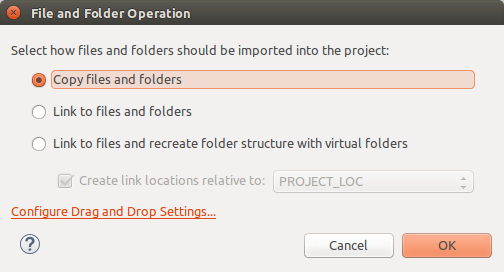
\includegraphics[width=0.8\textwidth] {janelaCopiarLinkar.png}
    \caption{Janela de importação de arquivos}
    \label{fig:janelaCopiarLinkar}
\end{figure}

\subsection{Inclusão de caminho na compilação}

Um outro modo de juntar as bibliotecas ao código fonte é adicionando seu caminho à compilação.
Com o projeto selecionado na janela lateral \emph{Project Explorer}, vá em \textbf{Project $>$ Properties $>$ Build $>$ GNU Compiler $>$ Directories} e clique em \emph{Add}, como na figura \ref{fig:incluindoDiretorio}.

\begin{figure}[!h]
\centering
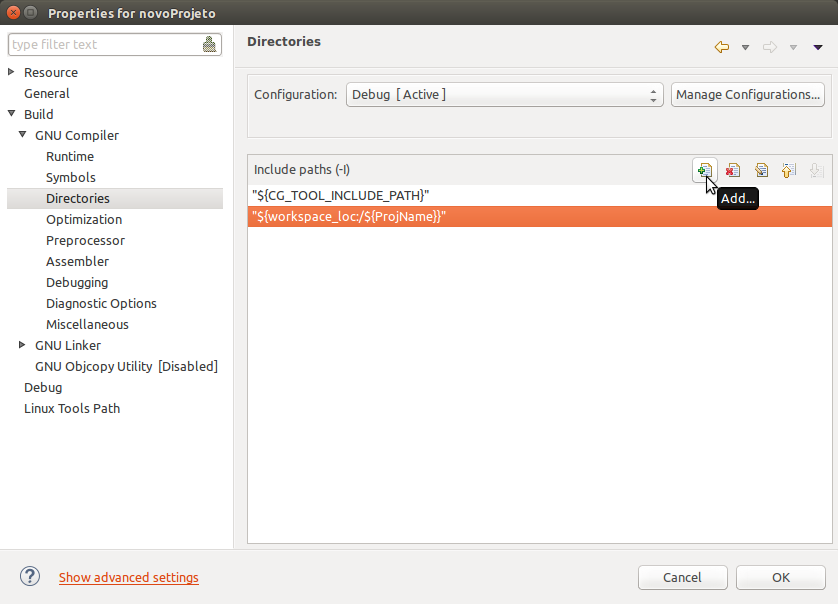
\includegraphics[width=1\textwidth] {incluindoDiretorio.png}
    \caption{Incluindo diretórios para compilação}
    \label{fig:incluindoDiretorio}
\end{figure}

Na janela aberta é possível digitar um caminho para o diretório ou arquivo, mas para prevenir erros existem os botões inferiores que abrirão uma navegação nos diretórios do sistema. Em \textbf{Workspace} é possível escolher o caminho para o diretório de um projeto ou de seus subdiretórios. Em \textbf{Variables} pode-se escolher o caminho armazenado em uma das variáveis de ambiente do projeto. E finalmente, em \textbf{Browse} é possível buscar um diretório navegando pelos arquivos do sistema.

\begin{figure}[H]
\centering
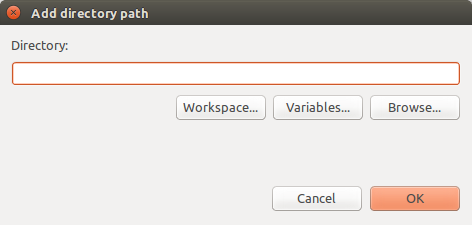
\includegraphics[width=0.8\textwidth] {incluindoDiretorio2.png}
    \caption{Escolhendo diretórios para incluir na compilação}
    \label{fig:incluindoDiretorio2}
\end{figure}

\section{TivaWare na ROM}

O TM4C1294NCPDT possui carregado na memória ROM uma parte da biblioteca de drivers do TivaWare. Isso possibilita a geração de um arquivo menor na hora da compilação, economizando memória de programa.

Para o uso das funções gravadas na ROM é necessário importar o arquivo de cabeçalho \emph{'driverlib/rom.h'} e ainda usar o prefixo \emph{'ROM\_'}  junto a função desejada. Por exemplo, para usar a função de configuração de clock do sistema $$SysCtlClockFreqSet()$$ carregada na ROM, esta deve ser chamada como $$ROM\_SysCtlClockFreqSet().$$

Porém, ao chamar tal função da ROM é possível que ela não seja encontrada na hora da compilação. Isso se deve ao fato de que nem todos os hardwares compatíveis com a TivaWare possuem uma memória ROM carregada com sua biblioteca ou mesmo não possua toda ela.
Tal problema é resolvido adicionando-se o arquivo de cabeçalho \emph{'driverlib/rom\_map.h'} e usando o prefixo \emph{'MAP\_'} junto às funções ao invés de \emph{'ROM\_'}. Para o exemplo da função de configuração de clock, a chamada seria feita da forma  $$MAP\_SysCtlClockFreqSet().$$ Esse arquivo de cabeçalho implementa uma estrutura que confere se a função usada existe na ROM do dispositivo para o qual o código será compilado e só assim a substitui. O prefixo de mapeamento pode ser usado em todas as chamadas de funções implementadas pela TivaWare.




